
\begin{figure}[h]
    \centering




\tikzset{every picture/.style={line width=0.75pt}} %set default line width to 0.75pt        

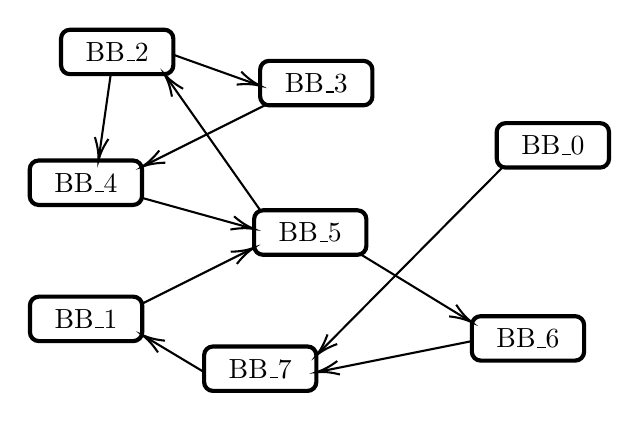
\begin{tikzpicture}[x=0.75pt,y=0.75pt,yscale=-1,xscale=1]
%uncomment if require: \path (0,385); %set diagram left start at 0, and has height of 385

%Rounded Rect [id:dp8950193773121069] 
\draw  [line width=1.5]  (251.91,67.28) .. controls (251.91,64.92) and (253.82,63) .. (256.19,63) -- (301.72,63) .. controls (304.08,63) and (306,64.92) .. (306,67.28) -- (306,80.12) .. controls (306,82.49) and (304.08,84.4) .. (301.72,84.4) -- (256.19,84.4) .. controls (253.82,84.4) and (251.91,82.49) .. (251.91,80.12) -- cycle ;
%Rounded Rect [id:dp9984058842626251] 
\draw  [line width=1.5]  (27,150.88) .. controls (27,148.51) and (28.92,146.6) .. (31.28,146.6) -- (76.81,146.6) .. controls (79.18,146.6) and (81.09,148.51) .. (81.09,150.88) -- (81.09,163.72) .. controls (81.09,166.08) and (79.18,168) .. (76.81,168) -- (31.28,168) .. controls (28.92,168) and (27,166.08) .. (27,163.72) -- cycle ;
%Rounded Rect [id:dp9856513256588806] 
\draw  [line width=1.5]  (137.91,37.28) .. controls (137.91,34.92) and (139.82,33) .. (142.19,33) -- (187.72,33) .. controls (190.08,33) and (192,34.92) .. (192,37.28) -- (192,50.12) .. controls (192,52.49) and (190.08,54.4) .. (187.72,54.4) -- (142.19,54.4) .. controls (139.82,54.4) and (137.91,52.49) .. (137.91,50.12) -- cycle ;
%Rounded Rect [id:dp901157696578387] 
\draw  [line width=1.5]  (26.91,85.28) .. controls (26.91,82.92) and (28.82,81) .. (31.19,81) -- (76.72,81) .. controls (79.08,81) and (81,82.92) .. (81,85.28) -- (81,98.12) .. controls (81,100.49) and (79.08,102.4) .. (76.72,102.4) -- (31.19,102.4) .. controls (28.82,102.4) and (26.91,100.49) .. (26.91,98.12) -- cycle ;
%Rounded Rect [id:dp24680170852961525] 
\draw  [line width=1.5]  (135,109.28) .. controls (135,106.92) and (136.92,105) .. (139.28,105) -- (184.81,105) .. controls (187.18,105) and (189.09,106.92) .. (189.09,109.28) -- (189.09,122.12) .. controls (189.09,124.49) and (187.18,126.4) .. (184.81,126.4) -- (139.28,126.4) .. controls (136.92,126.4) and (135,124.49) .. (135,122.12) -- cycle ;
%Rounded Rect [id:dp33862831913115987] 
\draw  [line width=1.5]  (239.91,160.28) .. controls (239.91,157.92) and (241.82,156) .. (244.19,156) -- (289.72,156) .. controls (292.08,156) and (294,157.92) .. (294,160.28) -- (294,173.12) .. controls (294,175.49) and (292.08,177.4) .. (289.72,177.4) -- (244.19,177.4) .. controls (241.82,177.4) and (239.91,175.49) .. (239.91,173.12) -- cycle ;
%Rounded Rect [id:dp1757835836146553] 
\draw  [line width=1.5]  (110.91,174.88) .. controls (110.91,172.51) and (112.82,170.6) .. (115.19,170.6) -- (160.72,170.6) .. controls (163.08,170.6) and (165,172.51) .. (165,174.88) -- (165,187.72) .. controls (165,190.08) and (163.08,192) .. (160.72,192) -- (115.19,192) .. controls (112.82,192) and (110.91,190.08) .. (110.91,187.72) -- cycle ;
%Rounded Rect [id:dp18264707725482388] 
\draw  [line width=1.5]  (42,22.28) .. controls (42,19.92) and (43.92,18) .. (46.28,18) -- (91.81,18) .. controls (94.18,18) and (96.09,19.92) .. (96.09,22.28) -- (96.09,35.12) .. controls (96.09,37.49) and (94.18,39.4) .. (91.81,39.4) -- (46.28,39.4) .. controls (43.92,39.4) and (42,37.49) .. (42,35.12) -- cycle ;
%Straight Lines [id:da3712867751572613] 
\draw    (138,105) -- (92.96,41.04) ;
\draw [shift={(91.81,39.4)}, rotate = 54.85] [color={rgb, 255:red, 0; green, 0; blue, 0 }  ][line width=0.75]    (10.93,-3.29) .. controls (6.95,-1.4) and (3.31,-0.3) .. (0,0) .. controls (3.31,0.3) and (6.95,1.4) .. (10.93,3.29)   ;
%Straight Lines [id:da3337276101977069] 
\draw    (66,39) -- (60.28,79.02) ;
\draw [shift={(60,81)}, rotate = 278.13] [color={rgb, 255:red, 0; green, 0; blue, 0 }  ][line width=0.75]    (10.93,-3.29) .. controls (6.95,-1.4) and (3.31,-0.3) .. (0,0) .. controls (3.31,0.3) and (6.95,1.4) .. (10.93,3.29)   ;
%Straight Lines [id:da3195921749278837] 
\draw    (96,30) -- (136.12,44.33) ;
\draw [shift={(138,45)}, rotate = 199.65] [color={rgb, 255:red, 0; green, 0; blue, 0 }  ][line width=0.75]    (10.93,-3.29) .. controls (6.95,-1.4) and (3.31,-0.3) .. (0,0) .. controls (3.31,0.3) and (6.95,1.4) .. (10.93,3.29)   ;
%Straight Lines [id:da3950293151484261] 
\draw    (141,54) -- (82.79,83.11) ;
\draw [shift={(81,84)}, rotate = 333.43] [color={rgb, 255:red, 0; green, 0; blue, 0 }  ][line width=0.75]    (10.93,-3.29) .. controls (6.95,-1.4) and (3.31,-0.3) .. (0,0) .. controls (3.31,0.3) and (6.95,1.4) .. (10.93,3.29)   ;
%Straight Lines [id:da7859903078227688] 
\draw    (81,99) -- (133.07,113.46) ;
\draw [shift={(135,114)}, rotate = 195.52] [color={rgb, 255:red, 0; green, 0; blue, 0 }  ][line width=0.75]    (10.93,-3.29) .. controls (6.95,-1.4) and (3.31,-0.3) .. (0,0) .. controls (3.31,0.3) and (6.95,1.4) .. (10.93,3.29)   ;
%Straight Lines [id:da22105063899115163] 
\draw    (81,150) -- (133.21,123.89) ;
\draw [shift={(135,123)}, rotate = 153.43] [color={rgb, 255:red, 0; green, 0; blue, 0 }  ][line width=0.75]    (10.93,-3.29) .. controls (6.95,-1.4) and (3.31,-0.3) .. (0,0) .. controls (3.31,0.3) and (6.95,1.4) .. (10.93,3.29)   ;
%Straight Lines [id:da18941500229563069] 
\draw    (111,183) -- (82.71,166.03) ;
\draw [shift={(81,165)}, rotate = 30.96] [color={rgb, 255:red, 0; green, 0; blue, 0 }  ][line width=0.75]    (10.93,-3.29) .. controls (6.95,-1.4) and (3.31,-0.3) .. (0,0) .. controls (3.31,0.3) and (6.95,1.4) .. (10.93,3.29)   ;
%Straight Lines [id:da8800586209378064] 
\draw    (186,126) -- (238.29,157.96) ;
\draw [shift={(240,159)}, rotate = 211.43] [color={rgb, 255:red, 0; green, 0; blue, 0 }  ][line width=0.75]    (10.93,-3.29) .. controls (6.95,-1.4) and (3.31,-0.3) .. (0,0) .. controls (3.31,0.3) and (6.95,1.4) .. (10.93,3.29)   ;
%Straight Lines [id:da8051529089918902] 
\draw    (240,168) -- (166.96,182.61) ;
\draw [shift={(165,183)}, rotate = 348.69] [color={rgb, 255:red, 0; green, 0; blue, 0 }  ][line width=0.75]    (10.93,-3.29) .. controls (6.95,-1.4) and (3.31,-0.3) .. (0,0) .. controls (3.31,0.3) and (6.95,1.4) .. (10.93,3.29)   ;
%Straight Lines [id:da13132970852441106] 
\draw    (255,84) -- (166.41,173.46) ;
\draw [shift={(165,174.88)}, rotate = 314.72] [color={rgb, 255:red, 0; green, 0; blue, 0 }  ][line width=0.75]    (10.93,-3.29) .. controls (6.95,-1.4) and (3.31,-0.3) .. (0,0) .. controls (3.31,0.3) and (6.95,1.4) .. (10.93,3.29)   ;

% Text Node
\draw (278.95,73.7) node   [align=left] {BB\_0};
% Text Node
\draw (54.05,157.3) node   [align=left] {BB\_1};
% Text Node
\draw (164.95,43.7) node   [align=left] {BB\_3};
% Text Node
\draw (53.95,91.7) node   [align=left] {BB\_4};
% Text Node
\draw (162.05,115.7) node   [align=left] {BB\_5};
% Text Node
\draw (266.95,166.7) node   [align=left] {BB\_6};
% Text Node
\draw (137.95,181.3) node   [align=left] {BB\_7};
% Text Node
\draw (69.05,28.7) node   [align=left] {BB\_2};


\end{tikzpicture}

    \caption{Block Diagram of the Entire SW Product}
    \label{complete_sw}
\end{figure}
